\documentclass[border=10pt]{standalone}
\usepackage[svgnames]{xcolor}
\usepackage{amsmath}
\usepackage{pgfplots}
\pgfplotsset{compat=newest}
\usepackage[sfdefault]{FiraSans}
\usepackage{FiraMono}
\renewcommand*\familydefault{\sfdefault}
\begin{document}
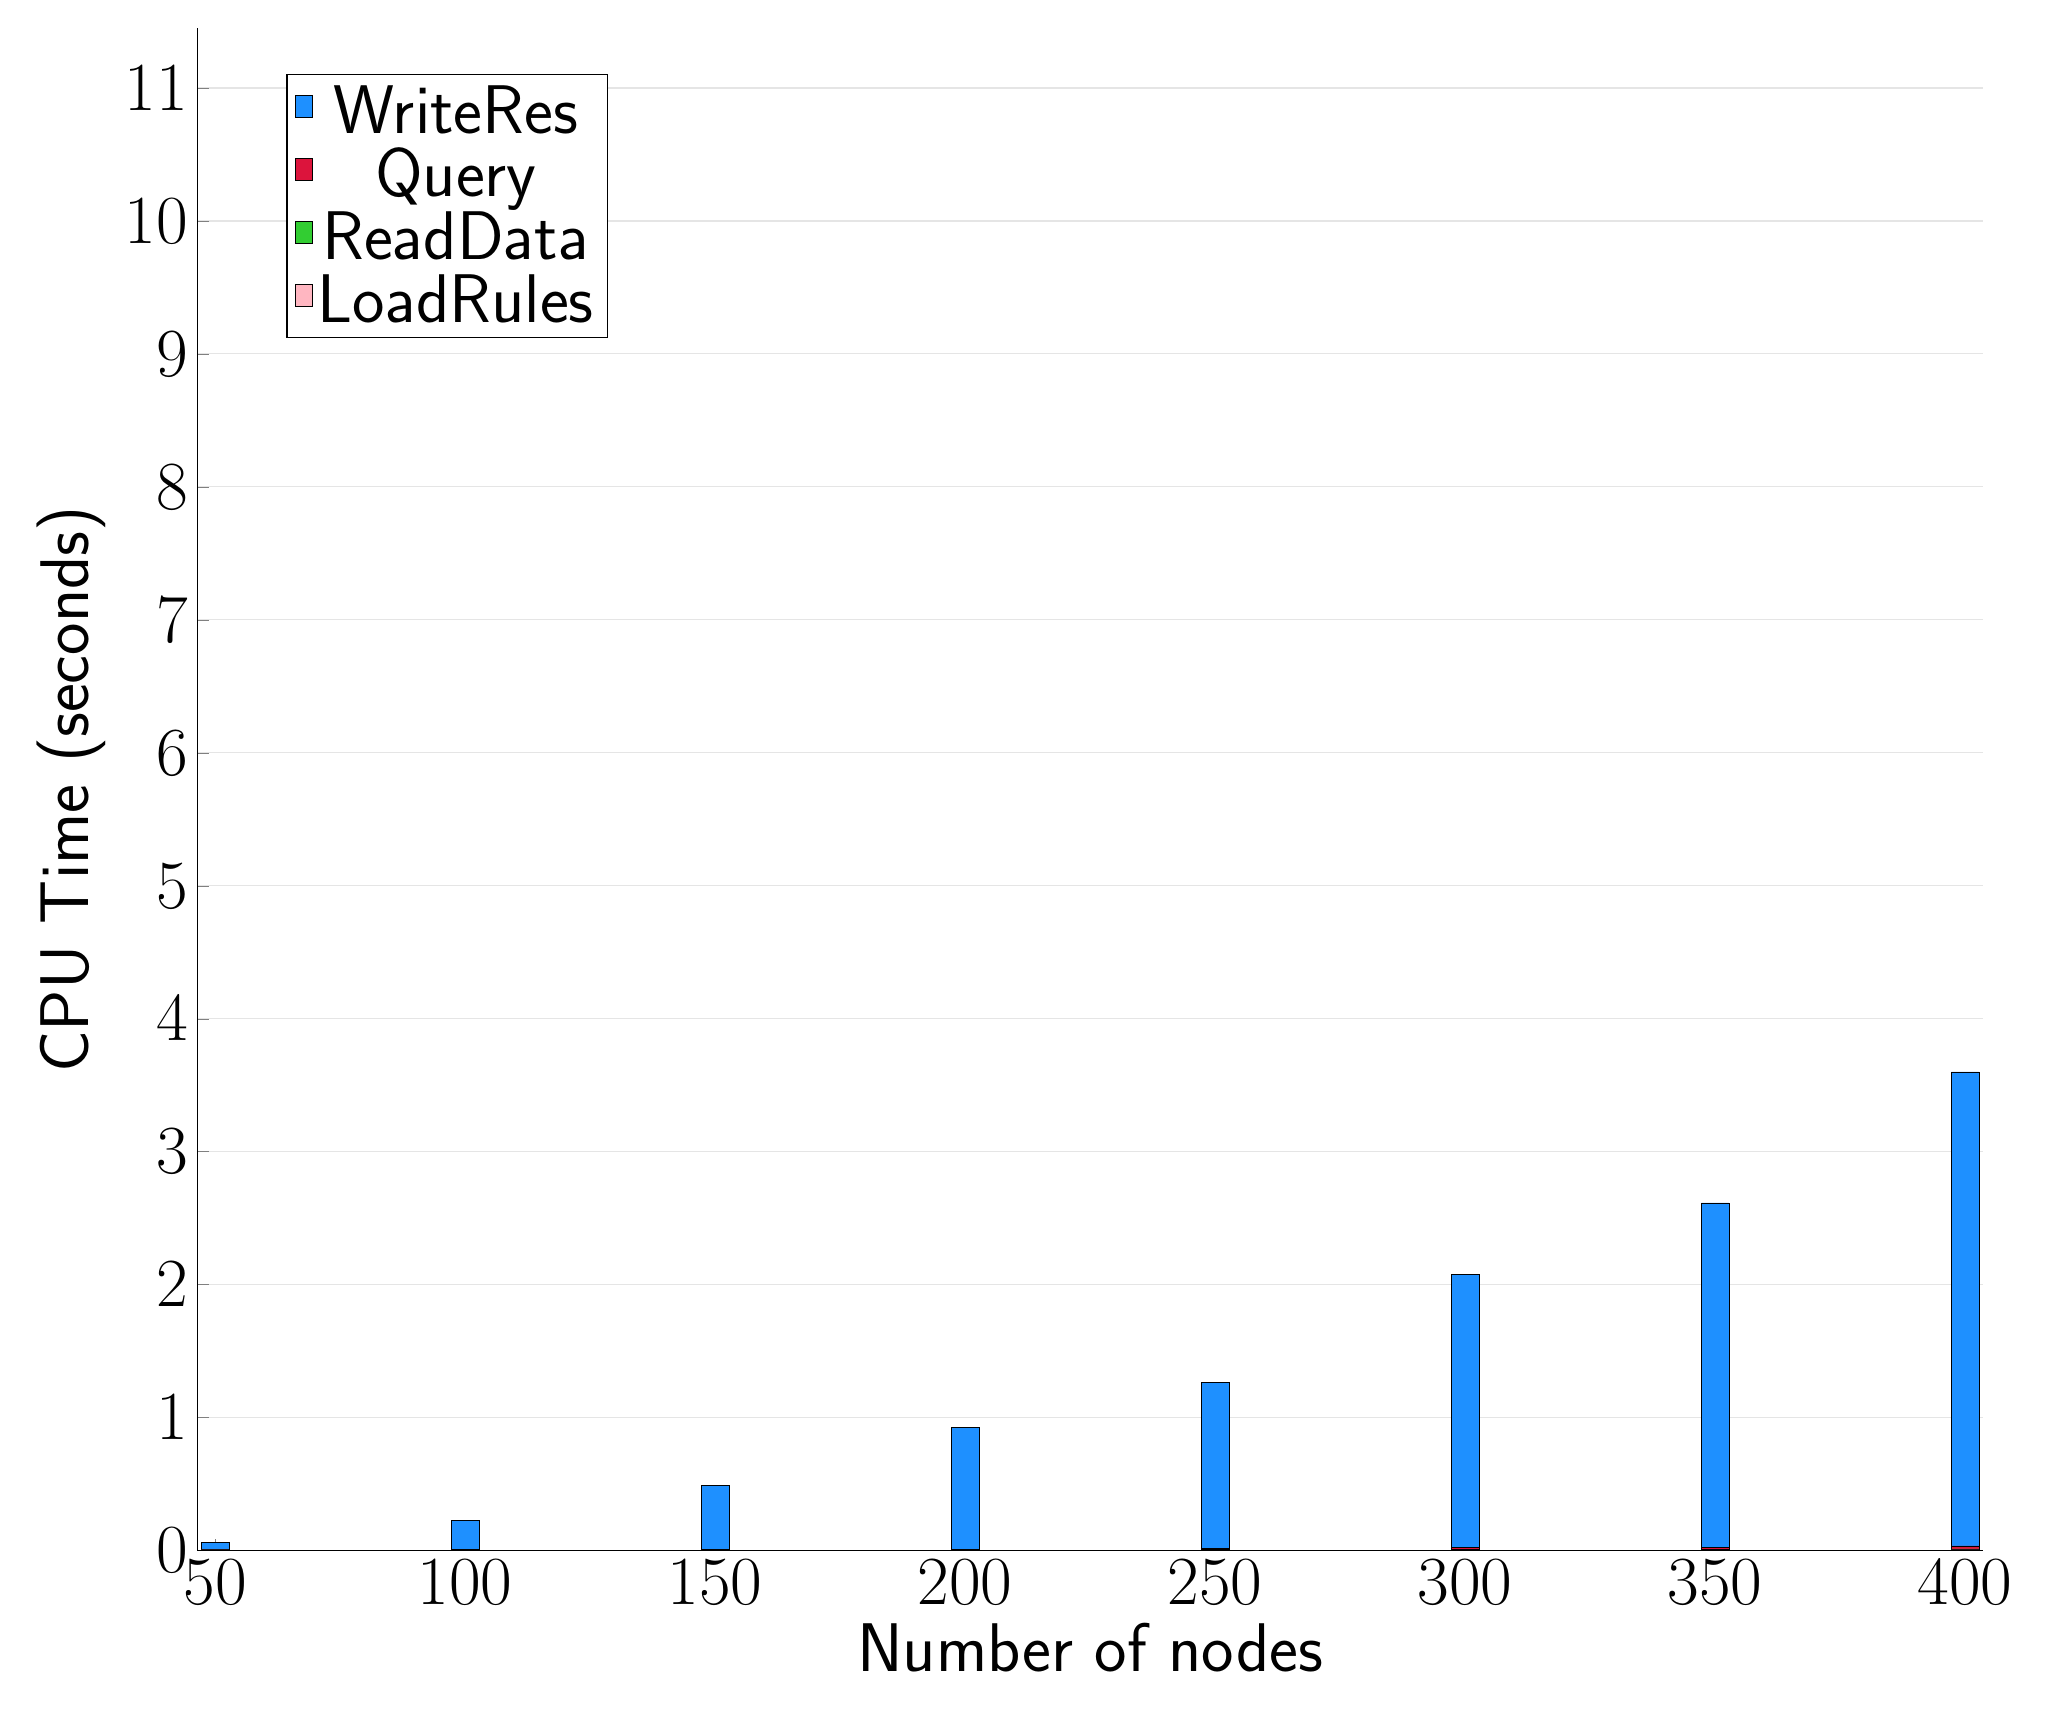
\begin{tikzpicture}
\begin{axis}[
   ybar stacked,
   width=2\textwidth,
   bar width=0.35cm,
   ymajorgrids, tick align=inside,
   major grid style={draw=gray!20},
   xtick=data,
   ymin=0, ymax=11.449559211730957,
   axis x line*=bottom,
   axis y line*=left,
   enlarge x limits=0.01,
   legend style={
       at={(0.23, 0.97)},
       anchor=north east,
       legend columns=1,
       font=\Huge,
   },
   ylabel={CPU Time (seconds)},
   xlabel={Number of nodes},
   label style={font=\Huge},
   tick label style={font=\Huge},
]
\addlegendimage{fill=DodgerBlue, draw=black, line width=0.2pt}
\addlegendentry{WriteRes}
\addlegendimage{fill=Crimson, draw=black, line width=0.2pt}
\addlegendentry{Query}
\addlegendimage{fill=LimeGreen, draw=black, line width=0.2pt}
\addlegendentry{ReadData}
\addlegendimage{fill=LightPink, draw=black, line width=0.2pt}
\addlegendentry{LoadRules}
\addplot +[fill=LightPink, draw=black, line width=0.2pt] coordinates {
(50, 0.005147000000000003)
(100, 0.004241333333333334)
(150, 0.004157)
(200, 0.0044856666666666664)
(250, 0.003969333333333333)
(300, 0.0039840000000000006)
(350, 0.003310000000000006)
(400, 0.005212666666666664)
};
\addplot +[fill=LimeGreen, draw=black, line width=0.2pt] coordinates {
(50, 0.0017709999999999965)
(100, 0.002603)
(150, 0.002866)
(200, 0.0037383333333333366)
(250, 0.004202999999999997)
(300, 0.0050156666666666665)
(350, 0.005759666666666663)
(400, 0.00821766666666667)
};
\addplot +[fill=Crimson, draw=black, line width=0.2pt] coordinates {
(50, 0.0004149999999999983)
(100, 0.0016509999999999969)
(150, 0.003371666666666663)
(200, 0.004230999999999996)
(250, 0.0077726666666666664)
(300, 0.013575666666666666)
(350, 0.014156666666666666)
(400, 0.02208033333333333)
};
\addplot +[fill=DodgerBlue, draw=black, line width=0.2pt] coordinates {
(50, 0.053276333333333335)
(100, 0.216944)
(150, 0.479125)
(200, 0.9122843333333334)
(250, 1.2498573333333332)
(300, 2.0578766666666666)
(350, 2.5914103333333336)
(400, 3.565314666666667)
};
\end{axis}
\end{tikzpicture}

\end{document}
